\documentclass[./einleitung.tex]{subfiles}
\usepackage{float}
\usepackage{float}
\usepackage{float}
\usepackage{float}
\usepackage{natbib}
\usepackage{listings}
\begin{document}
    \section{Die Nutzung des \acrshort{lsp}}
    \subsection{Installationsmöglichkeiten}
    Der \acrshort{lsp}-Server benötigt keine zusätzlichen Strukturen und kann direkt als Datei ausgeführt werden.
    Deshalb ist die normale Vorgehensweise das Ablegen des \acrshort{lsp}-Servers in einem Zentralen Server und das Hinzufügen des Pfades zu dem Umgebungsvariablen.
    Im Beispiel wurde die Datei zu `dmflsp' umbenannt, damit der Name genauer das Programm beschreibt und nicht mit anderen \acrshort{lsp}-Server kollidieren kann.\\
    \begin{figure}[h]
        \centering
        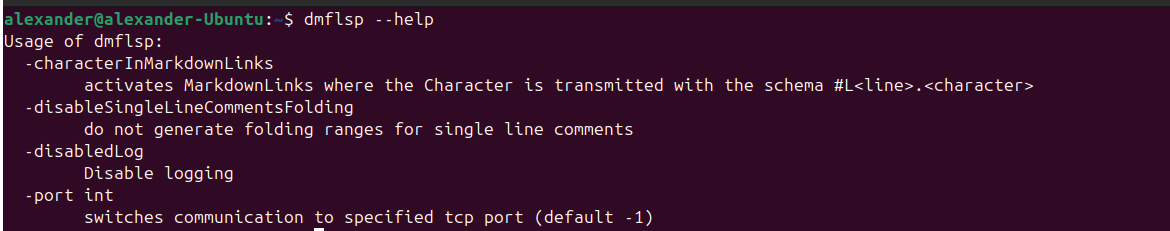
\includegraphics[width=\linewidth]{bilder/screenshot-lsp-help}
        \caption{Aufruf des \acrshort{cli} des \acrshort{lsp}-Servers}
        \label{fig:screenshot-lsp-help}
    \end{figure}\\
    Es gibt Editoren die eine native Anbindung eines \acrshort{lsp}-Servers ermöglichen.
        {\footnotesize TODO Zed Besspiel }
    \subsubsection{Intellij}
    Intellij unterstützt nur wenige \acrshort{lsp}-Funktionen ohne zusätzliche Plugins.
    Mit von `lsp4ij' können \acrshort{lsp}-Server direkt in der Oberfläche konfiguriert werden.\\
    \begin{figure}[h]
        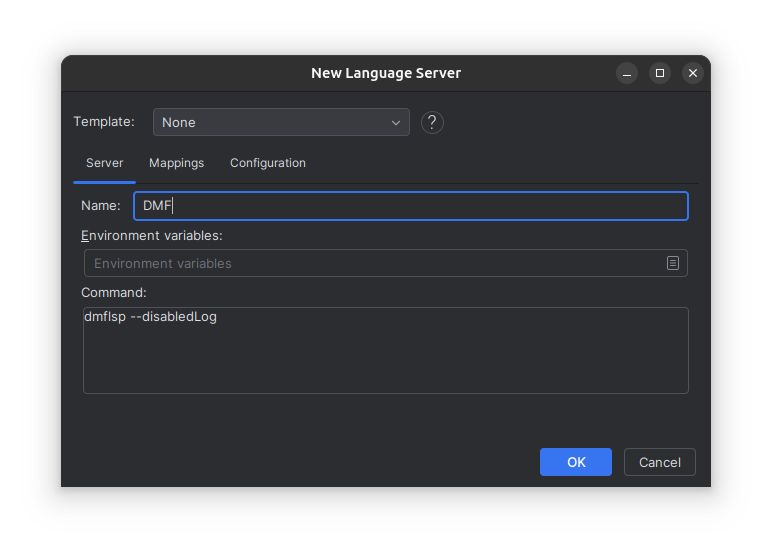
\includegraphics[width=\linewidth / 2]{bilder/screenshot-add-lsp-lsp4ij}
        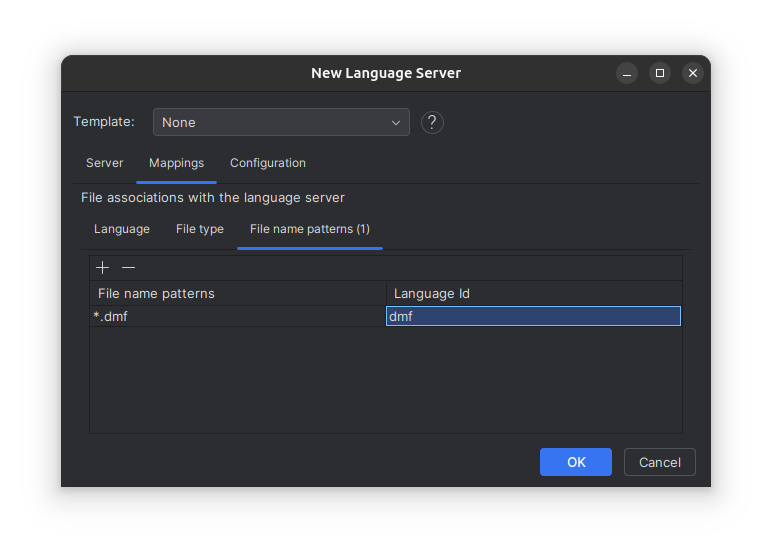
\includegraphics[width=\linewidth / 2]{bilder/screenshot-file-mapping}
        \caption{lsp4ij Konfiguration}
        \label{fig:screenshot-add-lsp-lsp4ij}
    \end{figure}\\
    Um diese Konfiguration automatisch anzulegen und den Dateien ein passendes Icon zu geben, kann das Intellij-Plugin für das \acrshort{dmf} verwendet werden.
    Es enthält die verschiedenen Versionen des Servers und kann sie automatisch an den konfigurierten Pfad ablegen.
    Der Pfad zum \acrshort{lsp}-Server kann entweder in den Einstellungen des Plugins oder über die Umgebungsvariable `DMF\_LSP' konfiguriert werden.

    \subsubsection{Visual Studio Code}
    Um den \acrshort{lsp}-Server in Visual Studio Code nutzen zu können, wird die Erweiterung für das \acrshort{dmf} benötigt.
    Dieses enthält die Logik zum Verbinden zum Server und die verschiedenen Versionen.
    Die benötigte Version kann direkt ausgeführt werden und benötigt keine zusätzliche Konfiguration.\\
    Im Gegensatz zu den bisherigen Konfigurationen nutzt die Visual Studio Code Erweiterung eine \acrshort{tcp}-Verbindung.


    \subsection{Funktionen im Editor}
    Während des Bearbeitens der Modelle können die Funktionen des \acrshort{lsp}-Servers genutzt werden.
    In diesem Abschnitt werden die Funktionen präsentiert.
    
    \subsubsection{Einfärbung des Textes}
    Mithilfe der semantischen Token kann der Editor den Text der Modelldatei einfärben.
    Da der Server nicht die Farbe, sondern nur die Funktion, vorgibt, wird der Text anhand der Einstellungen der Entwickler*innen eingefärbt.
    \begin{figure}[H]
        \centering
        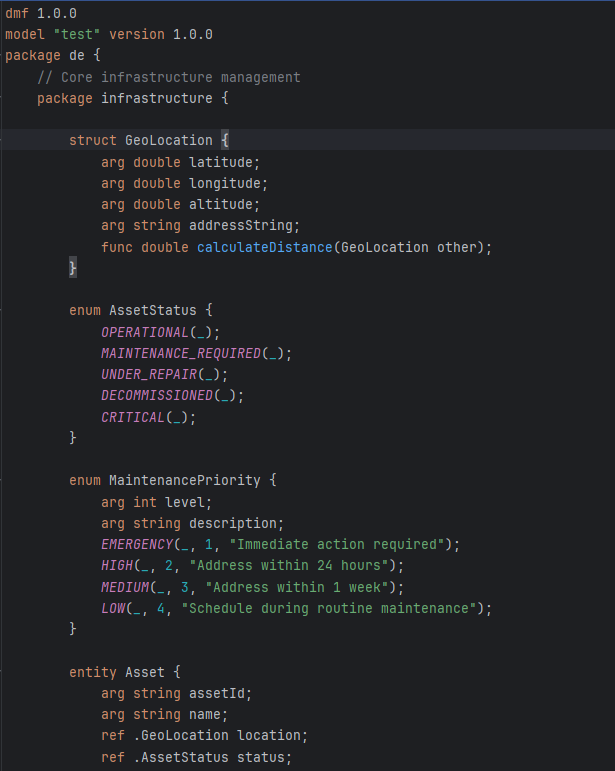
\includegraphics[width=\linewidth / 2 - 1em]{bilder/semanticIntellij}
        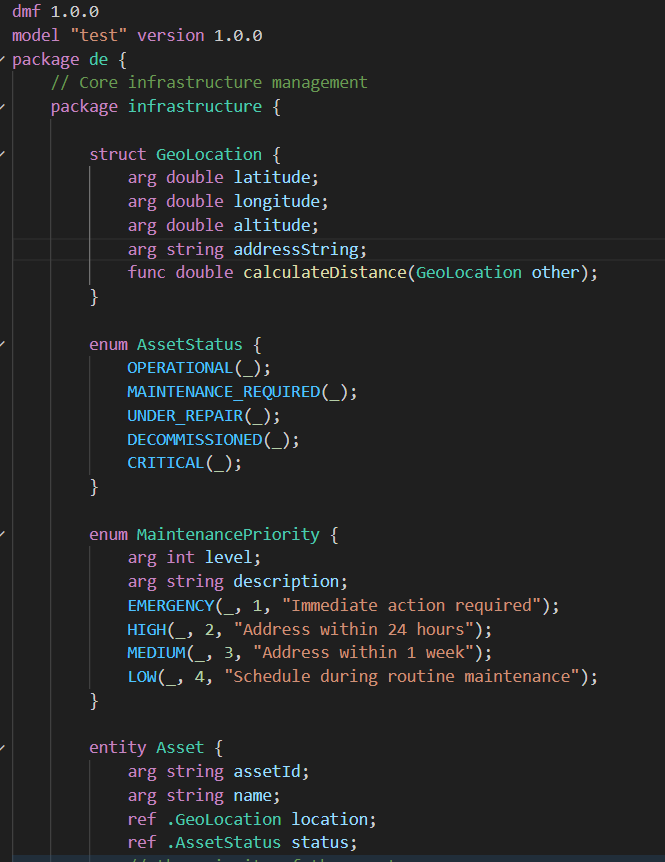
\includegraphics[width=\linewidth / 2 - 1em]{bilder/semanticVscode}
        \caption{Eingefärbte Modelldateien in Intellij und Visual Studio Code}
        \label{fig:semanticintellij}
    \end{figure}

    \subsubsection{Diagnosen}
    Wenn der Fehler in der Datei existieren werden diese automatisch im Editor markiert.
    Es wird auch eine Beschreibung und die detaillierte Beschreibung, welche auch im Generator ausgegeben wird, übertragen.\\
    Die Darstellung wird von der \acrshort{ide} übernommen.
    In Intellij und Visual Studio Code wird die Hover-Beschreibung zusätzlich angezeigt.\\
    \begin{figure}[hH]
        \centering
        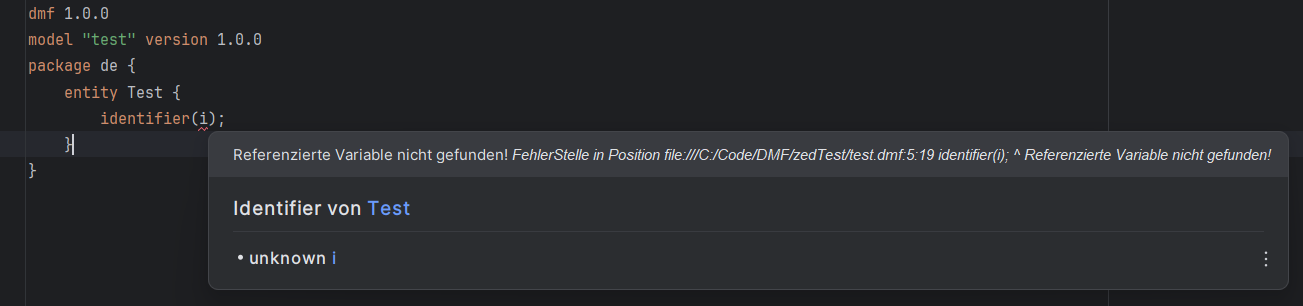
\includegraphics[keepaspectratio,height=8em]{bilder/markierung-fehler-intellij}
        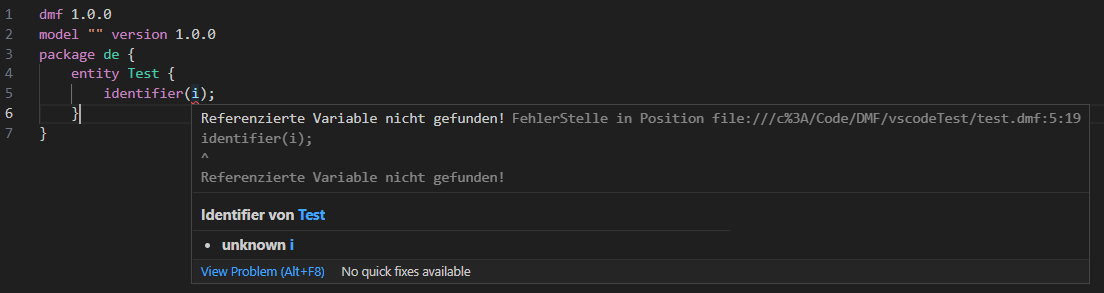
\includegraphics[keepaspectratio,height=8em]{bilder/markierung-fehler-vscode}
        \caption{Beispiele aus Intellij und Visual Studio Code}
        \label{fig:markierung-fehler-intellij}
    \end{figure}

    \subsubsection{Hover-Beschreibungen}
    Um Informationen über ein Element bereitzustellen, kann mit dem Mauszeiger über einem Element gehovered werden.
    Für alle PackageElemente, EntityIdentifier, Argumente, Referenzen, MultiReferenzen und Kommentare können Beschreibungen angezeigt werden.
    Mithilfe von Links in den Beschreibungen kann direkt zum erwähnten Element navigiert werden.
    \begin{figure}[H]
        \centering
        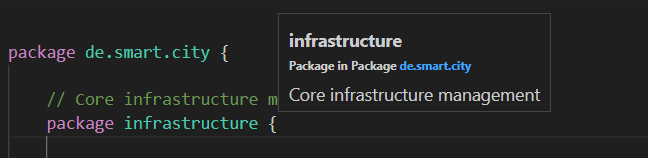
\includegraphics[height=5em]{bilder/hover-package}
        \caption{Beschreibung eines Package Elements}
        \label{fig:hover-package}
    \end{figure}
    Bei PackageElementen enthält die Beschreibung den Kommentar des Elements sowie das Package, in dem es liegt.
    \begin{figure}[H]
        \centering
        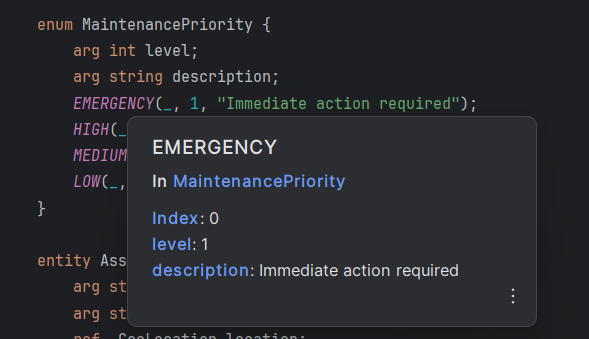
\includegraphics[height=7em]{bilder/hover-enum-entry}
        \caption{Beschreibung einer Enum Konstante ohne Kommentar}
        \label{fig:hover-enum-entry}
    \end{figure}
    Die Beschreibung von Enum Konstanten enthält das Enum, falls vorhanden den Kommentar und die Argumente des Enum mit den Werten der Konstante.
    Der erste Wert ist der Index, welcher in der Datenbank gespeichert wird.
    \begin{figure}[H]
        \centering
        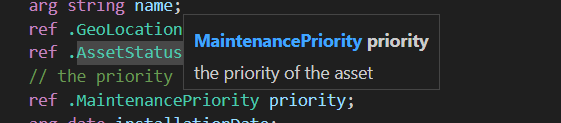
\includegraphics[height=5em]{bilder/hover-referenz}
        \caption{Beschreibung einer Referenz}
        \label{fig:hover-referenzen}
    \end{figure}
    Referenzen enthalten den Kommentar sowie den Typen und Namen der Variable.
    Argumente und MultiReferenzen verhalten sich gleich.
    \begin{figure}[H]
        \centering
        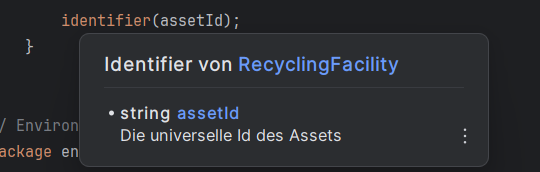
\includegraphics[height=7em]{bilder/hover-entity-identifier}
        \caption{Beschreibung eines Entity Identifiers}
        \label{fig:hover-entity-identifier}
    \end{figure}
    Bei einem Entity Identifier werden die referenzierten Variablen ihren Kommentaren angezeigt.

    \subsubsection{Referenzen}
    In den \acrshort{ide}s können die Referenzen aufgerufen werden.
    Der \acrshort{dmf}-\acrshort{lsp}-Server findet Referenzen, Deklarationen und Verwendungen in Parametern und EntityIdentifier.
    \begin{figure}[H]
        \centering
        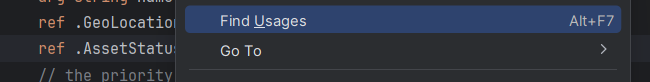
\includegraphics[height=2.5em]{bilder/callReferencen}
        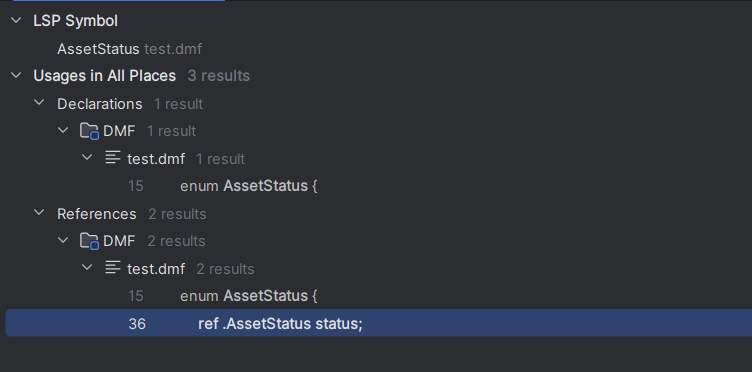
\includegraphics[height=6em]{bilder/referencen}
        \caption{Aufruf der Referenzen}
        \label{fig:callreferencen}
    \end{figure}

    \subsubsection{Faltbereiche}
    Damit Entwickler*innen in großen Dateien die Übersicht behalten können unterstützt der \acrshort{lsp}-Server die Übermittlung von Faltbereichen.
    Die Steuerung der Faltbereiche ist \acrshort{ide} spezifisch.
    \begin{figure}[H]
        \centering
        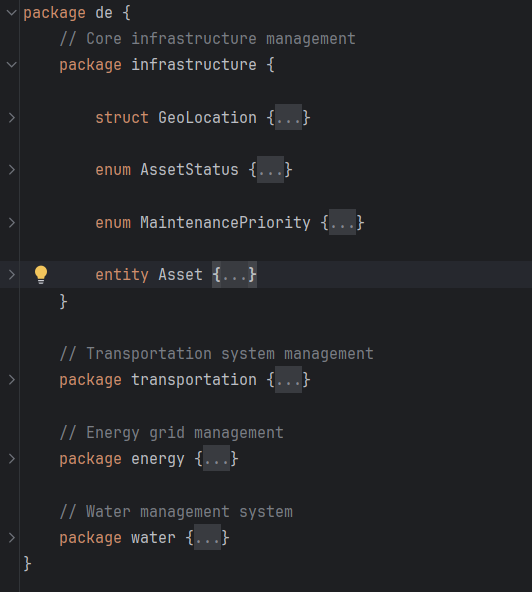
\includegraphics[height=15em]{bilder/faltbereich}
        \caption{Nutzung der Faltbereiche}
        \label{fig:faltbereich}
    \end{figure}

    \subsubsection{Auswahlbereiche}
    Damit die Entwickler*innen auch verschiedene Elemente gut Auswählen können, werden die Auswahlbereiche von \acrshort{lsp}-Server berechnet.
    \begin{figure}[H]
        \centering
        $\vimage{bilder/selection1.png}\vpointer
        \vimage{bilder/selection2.png}\vpointer
        \vimage{bilder/selection3.png}\vpointer
        \vimage{bilder/selection4.png}\vpointer
        \vimage{bilder/selection5.png}$
        \caption{Nutzung der Auswahlbereiche}
        \label{fig:selection}
    \end{figure}

    \section{Nutzung des \acrshort{dmf}}\label{sec:nutzung-des-dmf}
    Zum Darstellen der Benutzung des \acrshort{dmf} wird das Anlegen eines Projektes mit einem Java und einen Typescript Programm beschrieben.
    Es wird dafür das Modell aus dem Abschnitt \nameref{subsec:beispieldatei}.

    \begin{figure}[H]
        \caption{Dateiaufbau für ein Beispielprojekt}
        \dirtree{%
            .0 .
            .1 Modell.
            .2 domain.dmf.
            .2 base.dmf.
            .1 TSProjekt.
            .2 src.
            .3 de (Modell).
            .3 delegates (Delegates).
            .3 projekt (Projekt).
            .1 JDomain.
            .2 src/main/java (Delegates).
            .2 target/generated-sources/dmf (Modell).
            .1 JProjekt.
            .2 src/main/java (Projekt).
        }
        \label{fig:dirtree}
    \end{figure}

    \paragraph{Im Modell} Ordner wird das Modell abgelegt.
    Die Bereitstellung kann an die Organisation angepasst werden, da die restlichen Projekte per relativen Pfad auf die Datei zugreifen.
    Entscheidend ist dabei die Organisation der Git Repositories.
    Werden die verschiedenen Komponenten (Modell, Typescript Projekt, Java Projekt) in verschiedenen Repositories abgelegt, so handelt es sich um eine Poly-Repository Struktur. \cite{monorepo}
    Die Verwaltung der verschiedenen Repositories kann manuell durch Entwickler*innen oder durch Build Scripte gesteuert werden.
    Konträr zur Poly-Repository Struktur ist die Mono-Repository Struktur.
    Bei dieser werden alle Projekte in einem Repository verwaltet. \cite{monorepo}
    Hier entfällt die Synchronisation des Modells.
    \\\\
    In unserem Beispiel wird das vorher beschriebene Modell (siehe~\ref{subsec:beispieldatei}) zusammen mit einem Basismodell genutzt.
    \begin{lstlisting}[language=dmf, caption=Das Basismodell, label=lst:basismodell]
dmf 1.0.0
model "base" version 1.0.0

package de.base {
    interface IBeispiel {
        func string printBeispiel();
    }
}
    \end{lstlisting}

    \paragraph{Das Typescript Projekt} enthält sowohl die generierten Dateien als auch den Source Code des eigentlichen Projekts.
    Dies kann besonders in kleinen Projekten den Aufwand reduzieren.

    \paragraph{Das Java Projekt} wird in mehrere Artefakte unterteilt.
    Dies dient der Strukturierung von größeren Projekten und wurde exemplarisch genutzt, obwohl das Beispiel Projekt nur ein weiteres Artefakt besitzt.
    Innerhalb des JDomain Artefakts werden Modell und Delegates in verschiedene Ordner generiert, damit nur die Delegates von der Versionsverwaltung beachtet werden können und \acrshort{ide}s die Dateien richtig verwalten können.

    \subsection{Anlage des Typescript Projektes}\label{subsec:anlage-des-typescript-projektes}
    Das Beispiel Typescript Projekt nutzt die Bibliothek `Express' um einen kleinen Webserver zu implementieren.
    Ziel ist es die Verwendung des \acrshort{dmf} im Kontext einer simplen Restschnittstelle zu zeigen.\\
    Das Projekt wurde mithilfe der einer Anleitung von \citeauthor{initExpress} angelegt.\\
    Zuerst wird die `package.json'-Datei mithilfe der NPM-\acrshort{cli} angelegt.
    In ihr wird das Projekt beschrieben.
    Dazu gehören unter anderem der Name, Version, Abhängigkeiten und Ausführungskonfigurationen.\\
    Zu den Abhängigkeiten werden Dotenv, Typescript und Express hinzugefügt.
    Die Abhängigkeiten zu den Typen von Typescript und Express werden als `DevDependecies' hinzugefügt.
    So werden sie nur während der Entwicklung genutzt.\\
    Der nächste Schritt der Einrichtung ist die Konfiguration von Typescript.
    Es werden die Ordner für Source Code und Output sowie die beabsichtigte Version des JavaScript-Standards angegeben.\\
    Nun kann die Beispielimplementierung aus der Anleitung angelegt werden.
    Diese kann mit folgendem Befehl ausgeführt werden.
    \begin{lstlisting}{language=bash, caption=Start description Servers, label=lst:startExpress}
npx ts-node src/index.ts
    \end{lstlisting}
    Kann der Server aufgerufen werden, war die bisherige Anlage erfolgreich.
    Als nächstes kann das \acrshort{dmf} hinzugefügt werden.
    Dafür werden die Ausführungskonfigurationen erweitert.
    \begin{lstlisting}[language=json, caption=Ausführungskonfigurationen in package.json, label=lst:packageScripts]
"scripts": {
    "run": "npx ts-node src/index.ts",
    "build": "npm run generateModell && npm run generateDelegates && npx tsc",
    "start": "node dist/index.js",
    "generateModell": "generator --basePath ./src --mode ts --modelFile ../Modell/domain.dmf",
    "generateDelegates": "generator --basePath ./src --mode tsDelegates --modelFile ../Modell/domain.dmf",
  },
    \end{lstlisting}
    Es werden zwei neue Konfigurationen hinzugefügt: generateModell und generateDelegates.
    Sie rufen den Generator mit den Parametern für den Source Code Ordner, dem Pfad der Modelldatei und dem jeweiligen Generationsziel auf.
    Da die Konfigurationen in der Build Konfiguration eingebaut wurden, werden sie bei jedem Build automatisch ausgeführt.
    \paragraph{Die generierten Modelldateien} werden in den Ordnern nach ihrem Package Pfad abgelegt.
    Aus dem verwendeten Modell werden folgende Dateien generiert.
    \begin{lstlisting}[language=Typescript,caption=Aufgabe.ts, label=lst:aufgabeTs]
import { Beispiel } from "./Beispiel";
import * as delegate from "../../delegates/de/beispiel/AufgabeDelegate";

export class Aufgabe {
    beispiel: Beispiel;
    frage: string;
    antwort: string;
    id: number;

    constructor(frage: string, antwort: string, id: number, beispiel: Beispiel) {
        this.frage = frage;
        this.antwort = antwort;
        this.id = id;
        this.beispiel = beispiel;
    }

}
    \end{lstlisting}
    Bei der Aufgabe handelt es sich um eine Entity.
    Es werden alle Argumente und Referenzen (und evt. Funktionen) generiert.
    Typescript initialisiert Variablen nicht bei ihrer Definition.
    Sie müssen von Entwickler*innen gesetzt werden.
    Deshalb generiert das \acrshort{dmf} einen Konstruktor mit allen Variablen.
    \begin{lstlisting}[language=Typescript, caption=Beispiel.ts, label=lst:beispielTs]
import { IBeispiel } from "../base/IBeispiel";
import { BeispielTyp } from "./BeispielTyp";
import * as delegate from "../../delegates/de/beispiel/BeispielDelegate";

export class Beispiel implements IBeispiel {
    i: number;
    inhalt: string;
    typ: BeispielTyp;

    constructor(i: number, inhalt: string, typ: BeispielTyp) {
        this.i = i;
        this.inhalt = inhalt;
        this.typ = typ;
    }


    printBeispielMarkdown(): string {
        return delegate.printBeispielMarkdown(this);
    }

    printBeispiel(): string {
        return delegate.printBeispiel(this);
    }
}
    \end{lstlisting}
    In der Aufgabe wird das Struct Beispiel referenziert.
    Structs werden im Typescript Generator equivalent zu Entities generiert.
    Die Beispiel-Klasse demonstriert den Aufruf der Delegate Methoden.
    \begin{lstlisting}[language=Typescript, caption=BeispielTyp.ts, label=lst:beispielTypTs]
export enum BeispielTyp {
    CODE = 0,
    TEXT = 1
}

export interface BeispielTypDetails {

}


export const BeispielTypInfo : Record<BeispielTyp, BeispielTypDetails> = {
    [BeispielTyp.CODE]: {  },
    [BeispielTyp.TEXT]: {  },

}
    \end{lstlisting}
    Am Enum BeispielTyp kann die Emulation von weiteren Argumenten, ohne native Unterstützung, präsentiert werden, obwohl das Enum keine weiteren Argumente besitzt.
    Das eigentliche Enum besitzt nur Einträge mit den Datenbankindizes.
    Das Details-Interface würde eventuelle Argumente deklarieren.
    Im Info-Record werden die Enum Konstanten Details-Instanzen zugeordnet, welche die Werte aus dem Modell enthalten.\\
    Die Typen (Interface/Record) müssen für jede Sprache ersetzt werden.
    
    \paragraph{Die Delegate Funktionen} werden von den Modellklassen importiert und in den Funktionen der Modellklassen aufgerufen.
    \begin{lstlisting}[language=Typescript, caption=BeispielDelegate.ts, label=lst:beispielDelegateTs]
import {Beispiel} from "../../../de/beispiel/Beispiel";
import {BeispielTyp} from "../../../de/beispiel/BeispielTyp";


export function printBeispiel(caller: Beispiel): string {
    return `${caller.typ == BeispielTyp.TEXT ?
    "Text-" : "Code-"}Beispiel ${caller.i}`;
}

export function printBeispielMarkdown(caller: Beispiel): string {
    return `## Beispiel\n${caller.typ == BeispielTyp.TEXT ? "" :
    "```javascript\n"}${caller.inhalt}${caller.typ == BeispielTyp.TEXT ?
    "" : "\n```"}`;
}
    \end{lstlisting}
    In der Delegatedatei werden die Funktionen mit dem zusätzlichen Caller generiert.
    Die Inhalte der Funktionen müssen die Entwickler*innen selbstständig implementieren.
    \\\\
    Im Server kann nun ein neuer Endpunkt hinzugefügt werden, welcher eine Aufgabe mit einem Beispiel zu Markdown rendert und ausgibt.
    Die Aufgaben werden in einem Record gespeichert.
    In einem realen Projekt würden an dieser Stelle die Prozesse des Programms aufgerufen werden.
    \begin{lstlisting}[language=Typescript, caption=Neuer Endpunkt in index.ts, label=indexTs]
const aufgaben: Record<number, Aufgabe> = {
    1: new Aufgabe(
        "Was ist der Unterschied zwischen 'let' und 'const' in JavaScript?",
        "'let' erlaubt Variablen nach der Deklaration zu ändern, ...",
        1,
        new Beispiel(1,`let i = 1;\nconst ii = 2`, BeispielTyp.CODE)
    ),
    2: new Aufgabe(
        "Erkläre das Konzept der Vererbung in der objektorientierten Programmierung.",
        "Vererbung ist ein Mechanismus, bei dem eine Klasse die ...",
        2,
        new Beispiel(1,  `Ein Pferd ist genauso ein Tier wie ein Hund.`, BeispielTyp.TEXT)
    ),
}
app.get("/:id", (req: Request, res: Response) => {
    const id: number = Number(req.params["id"]);

    const aufgabe = aufgaben[id];

    if (!aufgabe) {
        res.status(404).send({
            error: 'Aufgabe not found'
        });
        return
    }
    res.setHeader('Content-Type', 'text/markdown');

    res.send(`# ${aufgabe.frage}\n${aufgabe.beispiel.printBeispielMarkdown()}`);
});
    \end{lstlisting}

    \subsection{Anlage des Java Projektes}\label{subsec:anlage-des-java-projektes}
    Für das Java Projekt wird Maven als Build Tool verwendet.
    Deshalb beginnt die Anlage der beiden Maven Artefakte mit der Anlage der `pom.xml'-Dateien.
    In ihnen werden die Namen, Versionen, die Plugins und Abhängigkeiten definiert.\\
    Im JDomain Artefakt kann jetzt die Ausführung des \acrshort{dmf}-Plugins hinzugefügt werden.
    \begin{lstlisting}[language=XML, caption=Konfiguration des \acrshort{dmf}-Plugins, label=lst:jdomainPlugins]
<build>
    <plugins>
        <plugin>
            <groupId>de.alex-brand.dmf</groupId>
            <artifactId>dmf-generator-plugin</artifactId>
            <version>0.0.1-SNAPSHOT</version>
            <executions>
                <execution>
                    <id>java-gen</id>
                    <goals>
                        <goal>generate-model</goal>
                    </goals>
                </execution>
                <execution>
                    <id>java-delegates-gen</id>
                    <goals>
                        <goal>generate-delegates</goal>
                    </goals>
                </execution>
                <execution>
                    <id>schema-gen</id>
                    <goals>
                        <goal>generate-model</goal>
                    </goals>
                    <configuration>
                        <zielsprache>sql</zielsprache>
                        <tempSources>./src/test/resources</tempSources>
                    </configuration>
                </execution>

            </executions>
            <configuration>
                <modelPath>../Modell/domain.dmf</modelPath>
            </configuration>
        </plugin>
    </plugins>
</build>
    \end{lstlisting}
    Mithilfe des Plugins werden die verschiedene Generationsziele in mehreren Ausführungen generiert.
    \paragraph{Die Modelldateien} befinden sich in einem Unterordner des `target'-Ordners.
    Im `target'-Ordner befinden sich alle temporären Dateien.
    \begin{lstlisting}[language=Java, caption=Beispiel.java, label=lst:beispielJava]
package de.beispiel;

import de.base.IBeispiel;
import java.util.Objects;

/**
 **/
public class Beispiel implements IBeispiel {
    protected static BeispielDelegate delegate = new BeispielDelegate();
    protected int i;
    protected String inhalt;
    protected BeispielTyp typ;

    public String printBeispiel(){
        return delegate.printBeispiel(this);
    }

    public String printBeispielMarkdown(){
        return delegate.printBeispielMarkdown(this);
    }

    public int getI() {
        return this.i;
    }

    public void setI(int i) {
        this.i = i;
    }

    public String getInhalt() {
        return this.inhalt;
    }

    public void setInhalt(String inhalt) {
        this.inhalt = inhalt;
    }
    public BeispielTyp getTyp() {
        return this.typ;
    }

    public void setTyp(BeispielTyp typ) {
        this.typ = typ;
    }


    @Override
    public boolean equals(Object o) {
        if (o == null || getClass() != o.getClass()) return false;
        Beispiel entity = (Beispiel) o;
        return Objects.equals(typ, entity.typ)  && Objects.equals(i, entity.i)  && Objects.equals(inhalt, entity.inhalt) ;
    }

    @Override
    public int hashCode() {
        return Objects.hash(typ, i, inhalt);
    }
}
    \end{lstlisting}
    Innerhalb der Java Klassen werden für jede Variable Getter und Setter Methoden generiert, um den Best Practices in Java zu folgen.\\
    Die Delegates werden in Java als Methoden in eigenen Klassen generiert.
    Um diese Methode aufzurufen wird in der Modellklasse eine statische Instanz der Delegateklasse erzeugt.
    In den Methoden der Modellklasse kann die Instanz der Delegateklasse aufgerufen werden.\\
    Die `equals' und die `hashCode' Methoden werden für jede generierte Klasse überschrieben.
    Sie bestimmen die Identität eines Objekts.
    Die für die Entities modellierte Identität wird auch in den Methoden beachtet.
    Deshalb werden bei Entities nur die Variablen des Identifiers in den Methoden genutzt.

    \begin{lstlisting}[language=Java, caption=BeispielTyp.java, label=lst:beispielTypJava]
package de.beispiel;

/**
 **/
public enum BeispielTyp {
    CODE(),
    TEXT();


    BeispielTyp(){

    }
}
    \end{lstlisting}
    Java Enum können zusätzliche Werte beinhalten.
    Würde das Enum BeispielTyp Argumente beinhalten, so würden diese als Variablen im Enum und im Konstruktor des Enums hinzugefügt werden.
    Die Werte einer Konstante werden direkt in die Deklaration der Konstante generiert.\\
    Datenbankindize werden nicht ins Java Enum generiert.
    
    \paragraph{Delegate Klassen}
    \begin{lstlisting}[language=Java, caption=BeispielDelegate.java, label=lst:beispielDelegateJava]
package de.beispiel;

/**
 * Delegate von Beispiel
 * Wird nur initial generiert.
 * Methoden müssen implementiert werden.
 **/
public class BeispielDelegate {

    public String printBeispiel(Beispiel caller){
        return "Beispiel: \n" + caller.getInhalt();
    }

    public String printBeispielMarkdown(Beispiel caller){
        return "";
    }
}
    \end{lstlisting}
    Die vorher erwähnten Delegateklassen werden in einen eigenen Ordner generiert.
    Sie enthalten alle Methode der ursprünglichen Klasse mit dem Modellobjekt als zusätzlichen Parameter.

    \paragraph{Java Programm}\mbox{}\\
    Um das angelegte Java Domain Modell zu nutzen wird das JProjekt Artefakt angelegt.
    Da es sich auch um ein Maven Projekt handelt, beginnt die Anlage mit der `pom.xml'-Datei.
    Das Java Programm soll eine ausführbare \acrshort{jar}-Datei erzeugen.
    Dafür werden Plugins hinzugefügt (siehe~\ref{sec:dateien-aus-dem-beispielprojekt}).\\
    Für das JDomain-Artefakt müssen zusätzlich die Abhängigkeiten angepasst werden.
    \begin{lstlisting}[language=XML, caption=Abhängigkeit zum JDomain Artefakt, label=lst:dependeciesJProjekt]
<dependencies>
    <dependency>
        <groupId>de.alex-brand</groupId>
        <artifactId>JDomain</artifactId>
        <version>1.0-SNAPSHOT</version>
    </dependency>
</dependencies>
    \end{lstlisting}
    Nun kann die Logik des Projektes implementiert werden.\\
    Es werden die gleichen Aufgaben wie im Typescript Projekt genutzt.
    Sie werden diesmal jedoch in einer Liste gespeichert.
    Für die Initialisierung der Aufgaben wurde eine eigene Methode implementiert.
    Durch diese Methoden könnte in einem größeren Projekt die Initialisierung überschrieben werden.\\
    Das Programm iteriert durch die Aufgaben.
    Der Nutzer deckt mit einer Eingabe die Antwort auf und springt zur nächsten Seite.
    Zur Ausgabe werden wird die Methode `Beispiel.printBeispiel()` genutzt, welche im BeispielDelegate implementiert wird.
    \begin{lstlisting}[language=Java, caption=Main.java, label=lst:mainJava]
public class Main {
    private static final List<Aufgabe> aufgaben = Arrays.asList(createAufgabe(1,
            "Was ist der Unterschied zwischen 'let' und 'const' in JavaScript?",
            "'let' erlaubt Variablen nach der Deklaration zu ändern, während 'const' nur eine einmalige Zuweisung erlaubt. Der Wert einer 'const' Variable kann nicht geändert werden, aber die Eigenschaften eines Objekts oder Arrays, das mit 'const' deklariert wurde, können geändert werden.",
            "let i = 1;\nconst ii = 2",
            BeispielTyp.CODE), createAufgabe(2,
            "Erkläre das Konzept der Vererbung in der objektorientierten Programmierung.",
            "Vererbung ist ein Mechanismus, bei dem eine Klasse die Eigenschaften und Methoden einer anderen Klasse erben kann. Die Klasse, die erbt, wird als abgeleitete Klasse oder Unterklasse bezeichnet, während die Klasse, von der geerbt wird, als Basisklasse oder Oberklasse bezeichnet wird. Durch Vererbung können gemeinsame Eigenschaften und Verhalten wiederverwendet werden.",
            "Ein Pferd ist genauso ein Tier wie ein Hund.",
            BeispielTyp.TEXT));

    public static void main(String[] args) {
        aufgaben.forEach(aufgabe -> {
            System.out.println();
            System.out.println("Frage: " + aufgabe.getFrage());
            System.out.println(aufgabe.getBeispiel().printBeispiel());
            try {
                System.in.read();
            } catch (IOException e) {
                throw new RuntimeException(e);
            }
            System.out.println("Antwort: "+aufgabe.getAntwort());
        });
    }

    private static Aufgabe createAufgabe(int id, String frage, String antwort, String beispiel, BeispielTyp beispielTyp) {
        Aufgabe aufgabe = new Aufgabe();
        aufgabe.setId(id);
        aufgabe.setFrage(frage);
        aufgabe.setAntwort(antwort);
        aufgabe.setBeispiel(new Beispiel());
        aufgabe.getBeispiel().setTyp(beispielTyp);
        aufgabe.getBeispiel().setInhalt(beispiel);
        return aufgabe;
    }
}
    \end{lstlisting}
\end{document}